\section{Iteration \#0 -- Evaluation Framework and Baselines}

This iteration describes the framework built for the project, which streamlines the evaluation process and discusses the implementations of the two evaluation baselines, Sequential Scan and Octree.

\subsection{Evaluation Framework}

\begin{table}
	\centering
	\makebox[\textwidth][c]{%
		\begin{tabular}{|r|r|l|l|l|l|l|l|l|l|l|l|}
			\hline
			\multicolumn{2}{|c}{} & \multicolumn{10}{|c|}{\textbf{Dimensions}} \\
			\hline
			\textbf{Structure} & \textbf{Operation} & 1 & 2 & 3 & 5 & 8 & 10 & 30 & 50 & 100 & 200 \\
			\hline
			\multirow{3}{*}{kdtree} & delete & 7.94729e-08& 7.94729e-08& 1.58946e-07& 1.58946e-07& 7.94729e-08& 0.0& 7.94729e-08& 7.94729e-08& 7.94729e-08& 7.94729e-08 \\
& insert & 7.94729e-08 & 1.58946e-07 & 1.58946e-07 & 7.94729e-08 & 7.94729e-08 & 1.58946e-07 & 7.94729e-08 & 7.94729e-08 & 1.58946e-07 & 7.94729e-08 \\ 
& pquery & 7.94729e-08 & 7.94729e-08 & 7.94729e-08 & 7.94729e-08 & 7.94729e-08 & 7.94729e-08 & 1.58946e-07 & 1.58946e-07 & 7.94729e-08 & 1.58946e-07 \\ 
\hline
\multirow{3}{*}{pseudo\_pyramid\_tree} & delete & 7.94729e-08& 7.94729e-08& 7.94729e-08& 7.94729e-08& 1.58946e-07& 7.94729e-08& 7.94729e-08& 7.94729e-08& 7.94729e-08& 7.94729e-08 \\
& insert & 1.58946e-07 & 7.94729e-08 & 1.58946e-07 & 7.94729e-08 & 7.94729e-08 & 7.94729e-08 & 7.94729e-08 & 7.94729e-08 & 7.94729e-08 & 7.94729e-08 \\ 
& pquery & 7.94729e-08 & 1.58946e-07 & 7.94729e-08 & 7.94729e-08 & 7.94729e-08 & 1.58946e-07 & 1.58946e-07 & 1.58946e-07 & 1.58946e-07 & 1.58946e-07 \\ 
\hline
\multirow{3}{*}{pyramid\_tree} & delete & 7.94729e-08& 7.94729e-08& 7.94729e-08& 7.94729e-08& 1.58946e-07& 7.94729e-08& 1.58946e-07& 7.94729e-08& 7.94729e-08& 1.58946e-07 \\
& insert & 7.94729e-08 & 7.94729e-08 & 1.58946e-07 & 7.94729e-08 & 1.58946e-07 & 1.58946e-07 & 7.94729e-08 & 7.94729e-08 & 7.94729e-08 & 1.58946e-07 \\ 
& pquery & 7.94729e-08 & 7.94729e-08 & 7.94729e-08 & 7.94729e-08 & 7.94729e-08 & 7.94729e-08 & 7.94729e-08 & 7.94729e-08 & 1.58946e-07 & 7.94729e-08 \\ 
\hline
		\end{tabular}
	}%

	\caption{TODO}
	\label{TODO}
\end{table}


Evaluation is a major part of the project and is performed multiple times at different stages of the project. It was decided a framework should be used to streamline this process and reduce the overall time it took generating the required measurements to perform the evaluation. It appeared there did not exist a tool tailored for this particular task, so one was implemented as part of the first iteration.

The evaluation framework defines the standard data used across the index structures, provide a way of loading point datasets and operation lists and feeding them to index structures. The framework executes the given operation lists on all specified structures, generating tables and plots containing the necessary performance measures described in Section \ref{sec:performance-measures}.

\begin{wrapfigure}[12]{r}{0.5\textwidth}
	\vspace{-40pt}
	\begin{center}
		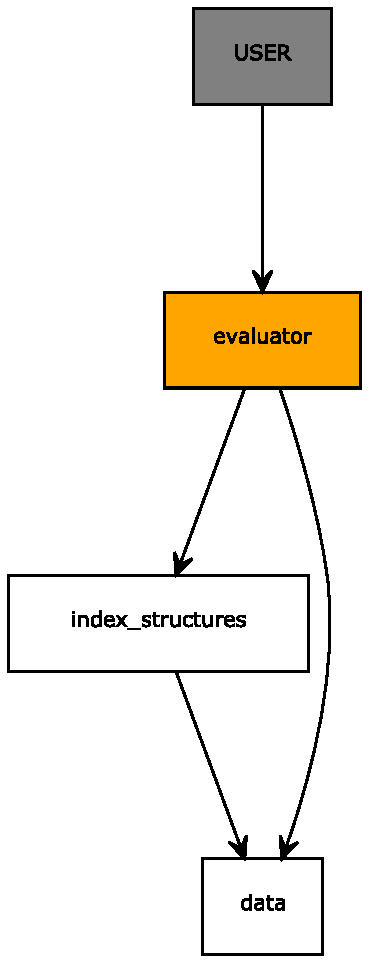
\includegraphics[scale=0.4]{figures/evaluation_framework.pdf}
	\end{center}
	\vspace{-20pt}
	\caption{Modules of Evaluation Framework}
	\label{fig:evaluation-framework}
\end{wrapfigure}

There are three core modules of the framework:
\begin{itemize}
	\item \texttt{data} -- library that contains standard data types used throughout framework and index structures, as well as dataset and test operation generators/loaders
	\item \texttt{index\_structure} -- library that contains all the index structures implemented throughout the project
	\item \texttt{evaluator} -- executable program that takes the index structures, operation lists and other options from the command line and runs a set of automated performance tests that produces timings and profiling (CPU and heap) information
\end{itemize}

The \texttt{evaluator} executable facilitates fast evaluation by allowing multiple index structures to be tested at once, using multiple tests operation lists (as described in Chapter \ref{chap:evaluation-outline}) at once. It stores timings in text files which are fed into bash and Gnuplot scripts to generate plots, which can be understood and incorporated into the report with ease. Figure \ref{fig:evaluation-framework} illustrates the modules of the framework, showing how user performing the performance evaluation only directly interacts with the \texttt{evaluator} executable.

The framework was created because performance analysis would be done very frequently, multiple times per iteration. Manually timing and profiling the code each time is time-consuming and error-prone. Putting more effort initially into creating a system that allows large sets of operations and index structures to be tested at once may save a significant amount of time , especially as many of these performance test are long and must be run multiple times to get averages.

Every index structure defined in the \texttt{index\_structures} module implement the \texttt{IndexStructure} interface, which has the following methods:
\begin{itemize}
	\item \texttt{loadPoints} -- bulk load a collection of points into structure
	\item \texttt{clear} -- remove all points from structure
	\item \texttt{insert} -- insert point into structure (if it's not already stored, see assumption (4) in Section \ref{sec:core-assumptions})
	\item \texttt{remove} -- remove point from structure
	\item \texttt{update} -- modify value of a specific point stored in the structure
	\item \texttt{pointExists} -- equivalent to a point query
\end{itemize}

\subsection{Baseline Implementations}
 
Sequential scan was implemented using the C++ container \texttt{std::vector}, a dynamically resizeable array.  Point queries are performed in $O(n)$ time, as the query iterates through the array sequentially until the given point is found or the end of the array is reached. Inserting a point is $O(1)$ as it is added to the end of the vector. However, Core Assumption (4) from Section \ref{sec:core-assumptions} states all points must be unique in a structure, meaning Sequential Scan must check if a given point exists before inserting it. This is a point query, meaning \texttt{insert} $\in O(n)$. \texttt{delete} is a standard array deletion, making it an $O(n)$ operation.

The octree variant implemented as a baseline is a bucket PR octree. This means the structure partitions the underlying data space into uniformly sized boxes, without using the points as pivots (unlike point quadtrees or kd-trees). It is a bucket octree because \textit{multiple} points can be stored in a single leaf node. The octree dynamically decomposes and composes spatial regions based on its current contents. When the number of points in a leaf node exceeds a certain number, say $M$, then the region represented by the leaf is sub-divided, creating $2^d$ children. The $M + 1$ points are then scattered across the children. Therefore, regions of space that contain more points are decomposed more and sparse regions of space have less granularity, meaning less nodes and memory overhead.

When a point is deleted from a leaf, the contents of the leaf and all of its siblings are checked. If all of these nodes are empty, they are removed and the sub-regions are combined into the original region again. If the now collapsed parent and all of its siblings are empty, then they are collapsed into their parent. This is repeatedly recursively until a parent is reached whose children contain at least one point.

\subsection{Compiler Optimisation}

GCC\footnote{GCC, the GNU Compiler Collection -- \url{http://gcc.gnu.org/}} was the C++ compiler used throughout development and analysis. GCC provides options to automatically modify the source code to make it more efficient on the target platform. There are multiple levels of optimisations, specifying using command line flags, going from 0 (\texttt{-O0} flag, no optimisation) to 3 (\texttt{-O3} flag, maximum optimisation). The default optimisation level is 0. In order to make the structures as fast as possible, level 3 optimisation was used to compile the structures. Table \ref{tab:compiler-optimisation} shows the average execution times for the three operations for each structure, using a 10D random uniformly distributed dataset with 10,000 points. The potential speed gains are huge. For example, the octree's point queries are approximately $6.5$ times faster, just by enabling level 3 optimisation.

\begin{table}
	\centering
	\begin{tabular}{|l|l|l|l|}
		\hline
		\textbf{Structure} & \textbf{Operation} & \texttt{-O0} & \texttt{-O3} \\
		\hline
		\multirow{ 4}{*}{\textbf{Sequential Scan}} & \textbf{Insert} & 1.33509 & 0.111372 \\
		 & \textbf{Delete} & 5.29548 & 0.623759 \\
		 & \textbf{Point Query} & 1.33468 & 0.111909 \\
		\hline
		\multirow{ 4}{*}{\textbf{Octree}} & \textbf{Insert} & 1.23108 & 0.243256 \\
		 & \textbf{Delete} & 0.73156 & 0.13589 \\
		 & \textbf{Point Query} & 0.559736 & 0.0860926 \\
		 \hline
	\end{tabular}
	\caption{Total Execution Time (in Seconds) of Structure Operations With and Without Compiler Optimisations (10D Randomly Uniform  Dataset, 10,000 points used)}
	\label{tab:compiler-optimisation}
\end{table}

While the potential performance boost can be high, there are some downsides to compiler optimisation. Using full optimisaiton can increase the size of the program binaries and it makes the program harder to debug, because the code is restructred and managed, making it difficult to get a method call trace \cite{gcc}. This also makes applications harder to profile. One could profile an application using no optimisation to avoid this issue, but there is no guarantee that functions/methods which are bottlenecks in the non-optimised binary are still bottlenecks in the fully optimised binary. Therefore, optimising the code to remove particular bottlenecks in the non-optimised version may have little, if no, impact on the fully optimised binary (that potentially still performs faster).

To summarise, full compiler optimisation will be used during performance analysis of the structures as the speed gains can be huge. Despite CPU profiling potentially being harder to understand and less useful on fully optimised binaries, this shall still be done over profiling the non-optimised binary because of the aforementioned reasons.